\documentclass[conference]{IEEEtran}
\IEEEoverridecommandlockouts
\usepackage{cite}
\usepackage{amsmath,amssymb,amsfonts}
\usepackage{graphicx}
\usepackage{textcomp}
\usepackage{xcolor}
\usepackage{booktabs}
\usepackage{url}
\usepackage{array}
\usepackage{multirow}
\usepackage{placeins}
\usepackage[hidelinks]{hyperref}

\def\BibTeX{{\rm B\kern-.05em{\sc i\kern-.025em b}\kern-.08em
    T\kern-.1667em\lower.7ex\hbox{E}\kern-.125emX}}

\begin{document}

\title{Benchmarking Supervised and Unsupervised Machine Learning for Network Intrusion Detection on UNSW-NB15}

\author{\IEEEauthorblockN{Douglas Felipe de Lima Silva}
\IEEEauthorblockA{
\textit{Instituto Metrópole Digital} \\
\textit{Universidade Federal do Rio Grande do Norte}\\
Natal, Brazil \\
pesquisadoug@gmail.com \\
ORCID: \href{https://orcid.org/0009-0007-9868-4891}{0009-0007-9868-4891}
}
}

\maketitle

\begin{abstract}
Network intrusion detection studies frequently rely on benchmark datasets, but aggregate predictive metrics can obscure attack-family behavior and computational trade-offs. This paper presents a reproducible benchmark of supervised and unsupervised machine-learning methods on the official predefined UNSW-NB15 train/test partition. The supervised study compares Dummy, Random Forest, XGBoost, Linear Support Vector Machine, and Multilayer Perceptron classifiers for binary attack detection, while the unsupervised study evaluates k-Means and DBSCAN on a bounded training-set sample after leakage-safe preprocessing and principal component analysis; \texttt{attack\_cat} and \texttt{id} are excluded from every model input, and data provenance is recorded via SHA-256 hashes. Using the FULL experimental profile, XGBoost obtained the numerically highest official held-out F1 score among non-baseline models (0.8943), with Random Forest (0.8907) and a Multilayer Perceptron (0.8893) close behind; bootstrap confidence intervals show that this ranking, while numerically consistent, is not separated by a wide margin. Attack-wise analysis shows that this aggregate performance conceals substantially lower recall on Fuzzers (0.8903 for XGBoost) than on other attack families, several of which are detected almost perfectly. The exploratory clustering analysis found that k-Means with $k=2$ achieved silhouette 0.3335, while an internally selected DBSCAN configuration produced 13 non-noise clusters with 3.18\% noise and silhouette 0.2544; post-hoc agreement with hidden labels remained low for both methods. All non-baseline models also exhibited a false positive rate above one quarter of normal traffic, underscoring that strong ROC-AUC and recall do not by themselves establish operational deployment readiness. These results support UNSW-NB15 as a controlled benchmark for classical machine learning while emphasizing that performance on this dataset does not establish operational network validity.
\end{abstract}

\begin{IEEEkeywords}
UNSW-NB15, intrusion detection, supervised learning, unsupervised learning, Random Forest, XGBoost, LinearSVC, MLP, k-Means, DBSCAN
\end{IEEEkeywords}

\section{Introduction}
Machine-learning-based network intrusion detection remains an active research area because network traffic is heterogeneous, imbalanced, and operationally costly to label. Public benchmark datasets are therefore useful for controlled comparison, but their use must be methodologically explicit: the dataset split, target semantics, leakage controls, preprocessing, metrics, and computational profile can materially affect conclusions. UNSW-NB15 was created as a modern intrusion-detection benchmark with normal traffic and nine attack families generated in a cyber-range environment \cite{moustafa2015unsw}. The dataset page maintained by UNSW provides the canonical source and data files used in this study \cite{unswDatasetPage}.

This work follows four research questions. RQ1 asks how Random Forest, XGBoost, a linear Support Vector Machine, and a Multilayer Perceptron compare for binary intrusion detection on the official UNSW-NB15 partition. RQ2 asks whether aggregate metrics hide differences across attack categories. RQ3 asks whether k-Means and DBSCAN reveal traffic structure related to normal and malicious behavior without using target labels during fitting. RQ4 asks what trade-offs exist among predictive performance, model size, training cost, and inference cost.

The contribution is not a new model architecture. Instead, the contribution is an auditable classical-ML benchmark that preserves the official UNSW-NB15 split, records file hashes, excludes post-hoc metadata from all model inputs, evaluates both aggregate and attack-wise behavior, and separates supervised classification from exploratory unsupervised structure analysis. This emphasis is important because prior analysis of UNSW-NB15 has highlighted dataset issues such as class imbalance and overlap that can complicate model interpretation \cite{moustafa2016evaluation}, a concern further quantified by subsequent overlap-aware modeling work \cite{zoghi2024overlap} and by classical feature-selection benchmarks evaluated on the same partition \cite{kasongo2020unsw}. More broadly, machine-learning intrusion detectors evaluated on closed, offline datasets are not guaranteed to generalize to operational deployment \cite{sommerpaxson2010closed}, which motivates the cautious, benchmark-scoped framing adopted throughout this paper.

\section{UNSW-NB15 Dataset}
UNSW-NB15 contains network traffic generated with a mixture of normal activity and attack scenarios. The benchmark used here follows the predefined partition distributed as \texttt{UNSW\_NB15\_training-set.csv} and \texttt{UNSW\_NB15\_testing-set.csv}. No random train/test split was created. Table~\ref{tab:dataset} summarizes the files used in this execution.

\begin{table}[htbp]
\caption{Dataset partition and integrity metadata}
\label{tab:dataset}
\centering
\resizebox{\columnwidth}{!}{
\begin{tabular}{lrrl}
\toprule
Partition & Rows & Columns & SHA-256 prefix \\
\midrule
Training & 175341 & 45 & bec7dd5ec88d \\
Testing & 82332 & 45 & 734fe6642edf \\
\bottomrule
\end{tabular}}
\end{table}

The supervised target is \texttt{label}, where 0 denotes normal traffic and 1 denotes attack traffic. The \texttt{attack\_cat} column is not a feature; it is retained only for post-hoc attack-wise recall analysis. The \texttt{id} column, when present, is also removed. After this exclusion, 42 input features remain, of which \texttt{proto}, \texttt{service}, and \texttt{state} are categorical and the remaining 39 are numeric.

\section{Methodology}
\subsection{Data Provenance and Integrity}
The pipeline first resolves the official CSV filenames under \texttt{data/raw/}. If they are absent, it downloads a SHA-256-verified public mirror of the predefined CSV partition while preserving the UNSW page as the canonical dataset source. This execution used the verified mirror and recorded the final SHA-256 values in \texttt{data/data\_manifest.json}. The validation step checks required columns, verifies that labels are a subset of \{0,1\}, confirms that training and testing schemas match, and warns if expected official row counts diverge.

\subsection{Feature Definition and Leakage Prevention}
The feature set is defined programmatically as all columns except \texttt{label}, \texttt{attack\_cat}, and \texttt{id}. This prevents target leakage and avoids using attack-family metadata during binary classification. The same exclusion is applied to supervised learning, permutation importance, clustering, and Streamlit inference. Categorical columns are detected from the expected UNSW-NB15 categorical fields plus any remaining object/category columns.

\subsection{Preprocessing}
Two supervised preprocessing strategies are used inside scikit-learn pipelines \cite{pedregosa2011scikit}. Tree-based models use numeric passthrough and one-hot encoding with \texttt{handle\_unknown="ignore"}. LinearSVC and MLP use standard scaling for numeric features and the same leakage-safe one-hot encoding for categorical features. Since preprocessing is nested inside the estimator pipeline, transformations are fitted only inside the corresponding training fold during cross-validation.

For clustering, a bounded training-set sample is transformed with standard scaling and dense one-hot encoding. Principal component analysis (PCA) is then applied both for the clustering representation and for two-dimensional visualization \cite{jolliffe2002pca}. The clustering fit never uses the official test set, \texttt{label}, or \texttt{attack\_cat}.

\subsection{Supervised Learning}
The supervised benchmark includes a Dummy baseline, Random Forest \cite{breiman2001random}, XGBoost \cite{chen2016xgboost}, LinearSVC based on support vector machines \cite{cortes1995svm}, and a Multilayer Perceptron classifier motivated by backpropagation-based neural networks \cite{rumelhart1986learning}. LinearSVC is used instead of a kernel SVM because the official training set has approximately 175 thousand records, making kernel methods substantially more expensive for this benchmark profile.

For Random Forest, XGBoost, SVM, and MLP, hyperparameters are selected with \texttt{RandomizedSearchCV}, three stratified folds, \texttt{scoring="f1"}, and \texttt{refit=True}. The official test set is not used for tuning. The FULL profile used in this study samples 15 configurations per non-baseline model, corresponding to 45 cross-validation fits, followed by refitting the selected configuration on the complete training partition. Random Forest searched \texttt{n\_estimators}$\in\{200,400,600\}$, \texttt{max\_depth}$\in\{\text{None},12,20,30\}$, \texttt{min\_samples\_split}$\in\{2,5,10\}$, \texttt{min\_samples\_leaf}$\in\{1,2,4\}$, \texttt{max\_features}$\in\{\text{sqrt},\text{log2}\}$, and \texttt{class\_weight}$\in\{\text{None},\text{balanced}\}$. XGBoost searched \texttt{n\_estimators}$\in\{200,400,600\}$, \texttt{max\_depth}$\in\{3,5,7,9\}$, \texttt{learning\_rate}$\in\{0.03,0.05,0.1,0.2\}$, \texttt{subsample}$\in\{0.7,0.85,1.0\}$, \texttt{colsample\_bytree}$\in\{0.7,0.85,1.0\}$, and \texttt{min\_child\_weight}$\in\{1,3,5\}$. LinearSVC searched $C$ log-uniformly on $[10^{-3},10^{2}]$ and \texttt{class\_weight}$\in\{\text{None},\text{balanced}\}$. MLP searched \texttt{hidden\_layer\_sizes}$\in\{(32),(64),(64,32),(128,64)\}$, \texttt{activation}$\in\{\text{relu},\text{tanh}\}$, $\alpha$ log-uniformly on $[10^{-5},10^{-2}]$, and the initial learning rate log-uniformly on $[10^{-4},10^{-2}]$. Table~\ref{tab:hyperparams} reports the selected configuration and its tuning-fold F1 for each model in the FULL run.

\begin{table}[htbp]
\caption{Selected hyperparameters after RandomizedSearchCV (FULL profile, 15 sampled configurations, three-fold tuning CV, F1 scoring)}
\label{tab:hyperparams}
\centering
\resizebox{\columnwidth}{!}{
\begin{tabular}{llr}
\toprule
Model & Selected hyperparameters & Tuning F1 \\
\midrule
RandomForest & n\_estimators=200, max\_depth=None, & 0.9694 \\
 & min\_samples\_split=5, min\_samples\_leaf=1, & \\
 & max\_features=log2 & \\
XGBoost & n\_estimators=600, max\_depth=9, & 0.9714 \\
 & learning\_rate=0.05, subsample=0.85, & \\
 & colsample\_bytree=0.85, min\_child\_weight=1 & \\
SVM & C=1.1436, class\_weight=None & 0.9545 \\
MLP & hidden\_layer\_sizes=(128,64), activation=relu, & 0.9615 \\
 & alpha=0.0011, learning\_rate\_init=0.00098 & \\
\bottomrule
\end{tabular}}
\end{table}

After tuning, a separate cross-validation pass evaluates the selected configurations on the training partition with five stratified folds (FULL profile) and random seed 43. This pass is a \emph{post-selection descriptive cross-validation}: it should not be interpreted as an unbiased independent estimate of generalization performance, because the same training partition informed both hyperparameter selection and this evaluation.

\subsection{Evaluation Metrics}
The official test-set evaluation reports accuracy, balanced accuracy, precision, recall/detection rate, F1, ROC-AUC, PR-AUC, Matthews correlation coefficient (MCC), false positive rate (FPR), final fit time, median per-record inference time, and serialized model size. PR-AUC is included because precision-recall analysis is informative under class imbalance \cite{davis2006pr}. FPR is defined as false positives divided by the number of normal records, i.e., records where \texttt{label=0}. Median inference time is measured by timing 30 full-batch \texttt{predict} calls (FULL profile) over the entire official test set and dividing the median total time by the number of test records, with no explicit warm-up iteration excluded; Random Forest and XGBoost use internal multi-threaded prediction (\texttt{n\_jobs=-1}), while LinearSVC, MLP, and the Dummy baseline predict on a single thread, so cross-model timing comparisons partly reflect this difference in parallelism rather than pure per-model cost alone. Bootstrap confidence intervals are computed independently for every supervised model by resampling each model's fixed official-test predictions 1500 times (FULL profile); models are not retrained during bootstrap.

\subsection{Attack-wise Analysis}
The classification task remains binary. After predictions are produced, the test records with \texttt{label=1} are grouped by \texttt{attack\_cat}. For each model and attack family, the pipeline reports the number of attack records, detected attacks, missed attacks, and recall. This analysis directly addresses whether aggregate metrics hide attack-family-specific behavior.

\subsection{Unsupervised Learning}
The unsupervised component is exploratory and never uses \texttt{label} or \texttt{attack\_cat} to fit a model; both are used only for post-hoc comparison. k-Means \cite{macqueen1967kmeans} is evaluated for $k=2$ through $k=10$ on the PCA-transformed representation, with $k=2$ retained as the primary binary-structure comparison. DBSCAN \cite{ester1996dbscan} candidates use \texttt{min\_samples} in \{5, 10, 20\}; candidate \texttt{eps} values are derived from the 0.80, 0.85, 0.90, and 0.95 quantiles of k-nearest-neighbor distances computed in the same PCA space. DBSCAN selection uses only internal information: at least two non-noise clusters, at least 100 non-noise observations, higher silhouette computed after excluding noise points, and lower noise fraction as a secondary criterion; hidden labels never participate in candidate selection. Adjusted Rand Index (ARI) and Normalized Mutual Information (NMI) are reported only as post-hoc external comparisons against hidden labels. Both algorithms are fitted on the full multi-dimensional PCA representation retained for the profile; the accompanying two-dimensional scatter plots shown later use only the first two principal components (PC1, PC2) for visualization and do not represent the space used for fitting.

\subsection{Reproducibility}
The implementation writes CSV tables, PNG figures, serialized models, feature schemas, data manifests, and experiment manifests. The FULL run reported in this paper used Python 3.12.0 with NumPy 2.5.3, pandas 3.0.5, scikit-learn 1.9.1, XGBoost 3.4.1, SciPy 1.18.1, matplotlib 3.11.2, and joblib 1.6.0, executed on an Intel Core i7-14700K (20 physical / 28 logical cores) with 32~GB RAM running Windows 11 Pro (64-bit). Random seed 42 is used for sampling and model construction where supported; the descriptive cross-validation pass uses seed 43. The FULL run itself predates version control; the repository state that archives the exact code, configuration, and results reported here, together with this manuscript, corresponds to Git revision \texttt{0c44383212677a3dfc4facb3a69a495bfce412f4}.

\section{Results}
\subsection{Cross-validation}
Table~\ref{tab:cv} summarizes the post-selection descriptive training-set cross-validation of the selected configurations (FULL profile, five stratified folds). XGBoost achieved the numerically highest mean CV F1 (0.9727), followed by Random Forest (0.9705) and MLP (0.9618). The Dummy baseline has high recall because it predicts the majority attack class in the training partition, but its MCC is 0.0 and ROC-AUC is 0.5, as expected for a label-blind classifier.

\begin{table}[htbp]
\caption{Post-selection descriptive training-set cross-validation of selected configurations}
\label{tab:cv}
\centering
\resizebox{\columnwidth}{!}{
\begin{tabular}{lrrrr}
\toprule
Model & F1 mean & ROC-AUC & PR-AUC & MCC \\
\midrule
XGBoost & 0.9727 & 0.9947 & 0.9975 & 0.9133 \\
RandomForest & 0.9705 & 0.9939 & 0.9970 & 0.9060 \\
MLP & 0.9618 & 0.9906 & 0.9955 & 0.8785 \\
SVM & 0.9546 & 0.9840 & 0.9915 & 0.8526 \\
Dummy & 0.8100 & 0.5000 & 0.6806 & 0.0000 \\
\bottomrule
\end{tabular}}
\end{table}

\subsection{Official Test-set Benchmark}
Table~\ref{tab:test} reports official held-out test metrics for the FULL run. XGBoost obtained the numerically highest F1 (0.8943), ROC-AUC (0.9837), and PR-AUC (0.9881) among all models, with MCC 0.7551. Random Forest (F1 0.8907, MCC 0.7468) and MLP (F1 0.8893, MCC 0.7417) were close behind, while LinearSVC trailed with F1 0.8525 and MCC 0.6504. Fig.~\ref{fig:benchmark} shows the main held-out benchmark, and Fig.~\ref{fig:rocpr} summarizes ROC and precision-recall behavior for all five models.

\begin{table*}[t]
\caption{Official test-set supervised benchmark. Acc.\ = Accuracy, Bal.\ Acc.\ = Balanced Accuracy, Prec.\ = Precision, Rec.\ = Recall, ROC and PR denote ROC-AUC and PR-AUC.}
\label{tab:test}
\centering
\resizebox{\textwidth}{!}{
\begin{tabular}{lrrrrrrrrr}
\toprule
Model & Acc. & Bal. Acc. & Prec. & Rec. & F1 & ROC & PR & MCC & FPR \\
\midrule
XGBoost & 0.8720 & 0.8594 & 0.8199 & 0.9835 & 0.8943 & 0.9837 & 0.9881 & 0.7551 & 0.2646 \\
RandomForest & 0.8666 & 0.8530 & 0.8115 & 0.9870 & 0.8907 & 0.9804 & 0.9849 & 0.7468 & 0.2809 \\
MLP & 0.8671 & 0.8555 & 0.8210 & 0.9701 & 0.8893 & 0.9747 & 0.9812 & 0.7417 & 0.2591 \\
SVM & 0.8123 & 0.7929 & 0.7513 & 0.9852 & 0.8525 & 0.9543 & 0.9647 & 0.6504 & 0.3995 \\
Dummy & 0.5506 & 0.5000 & 0.5506 & 1.0000 & 0.7102 & 0.5000 & 0.5506 & 0.0000 & 1.0000 \\
\bottomrule
\end{tabular}}
\end{table*}

\begin{figure}[htbp]
\centerline{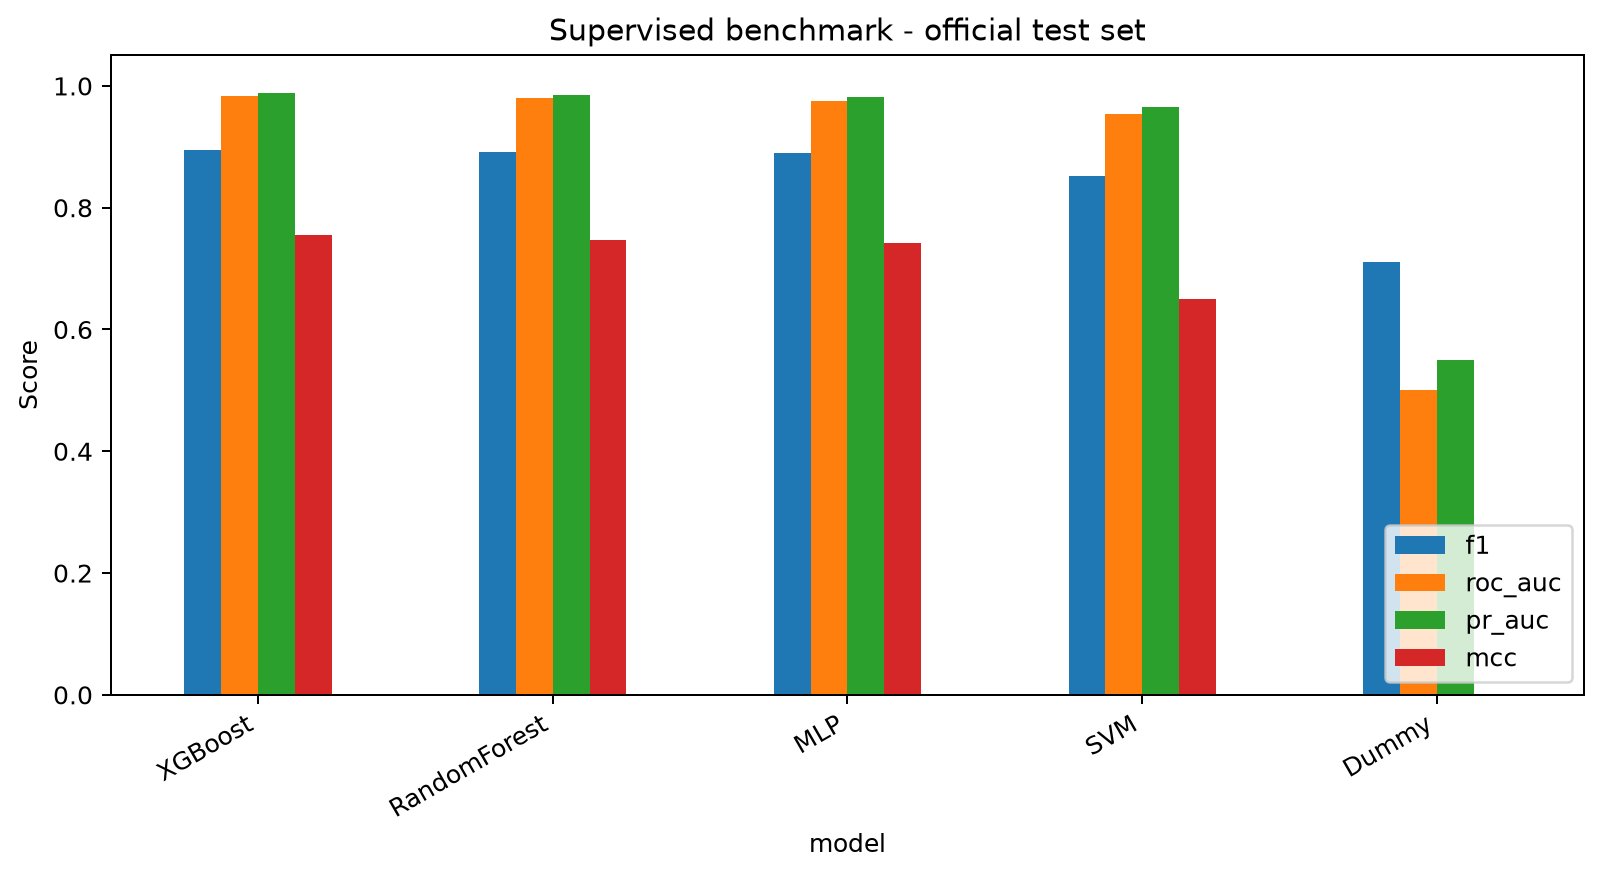
\includegraphics[width=\columnwidth]{figures/05_supervised_benchmark.png}}
\caption{Official test-set supervised benchmark for F1, ROC-AUC, PR-AUC, and MCC.}
\label{fig:benchmark}
\end{figure}

\begin{figure*}[t]
\centering
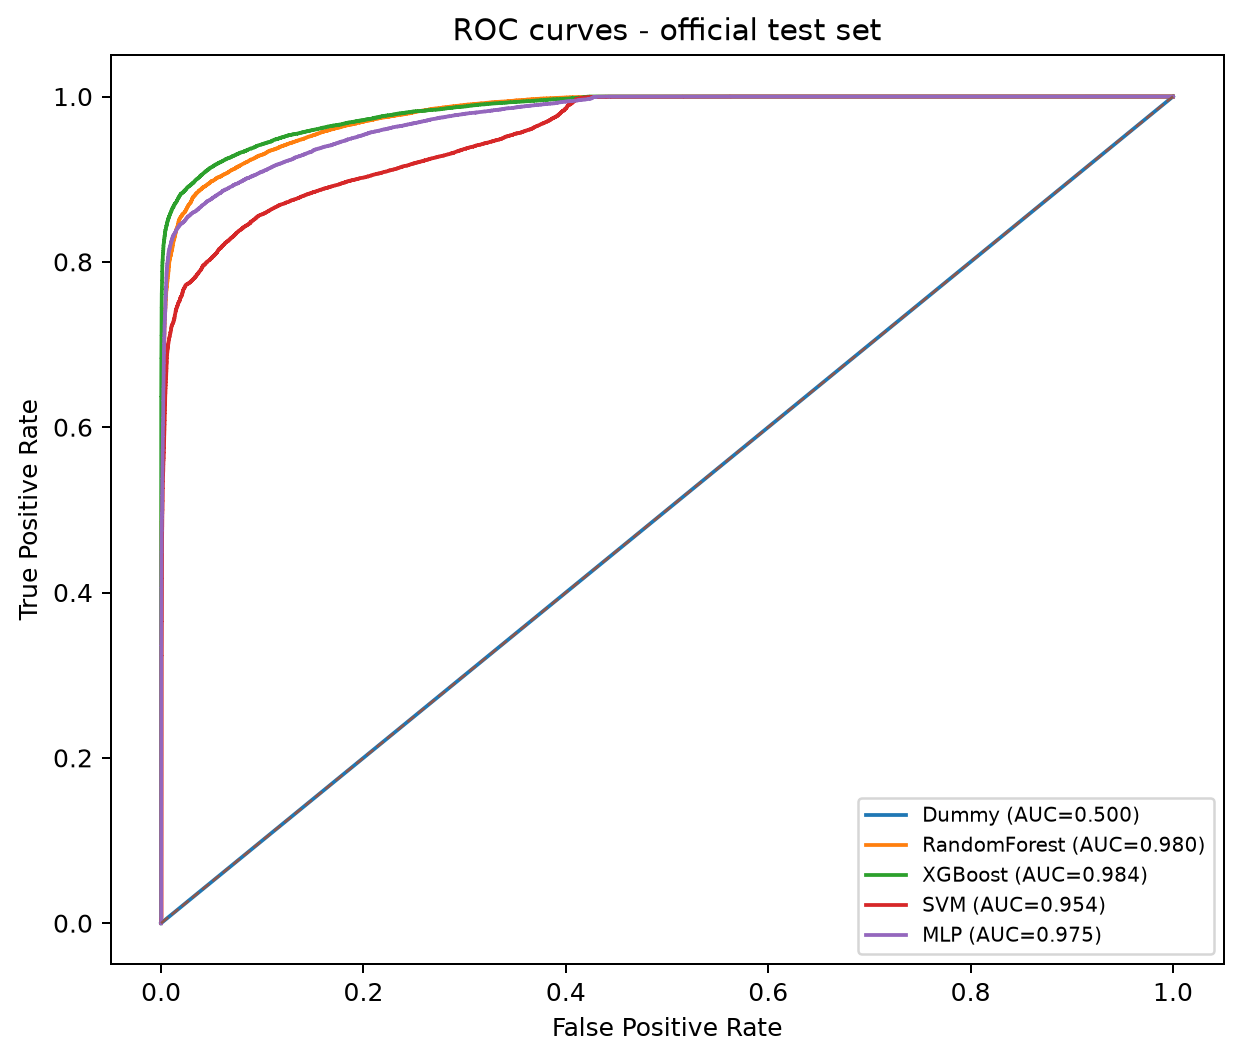
\includegraphics[width=0.48\textwidth]{figures/03_roc_curves.png}
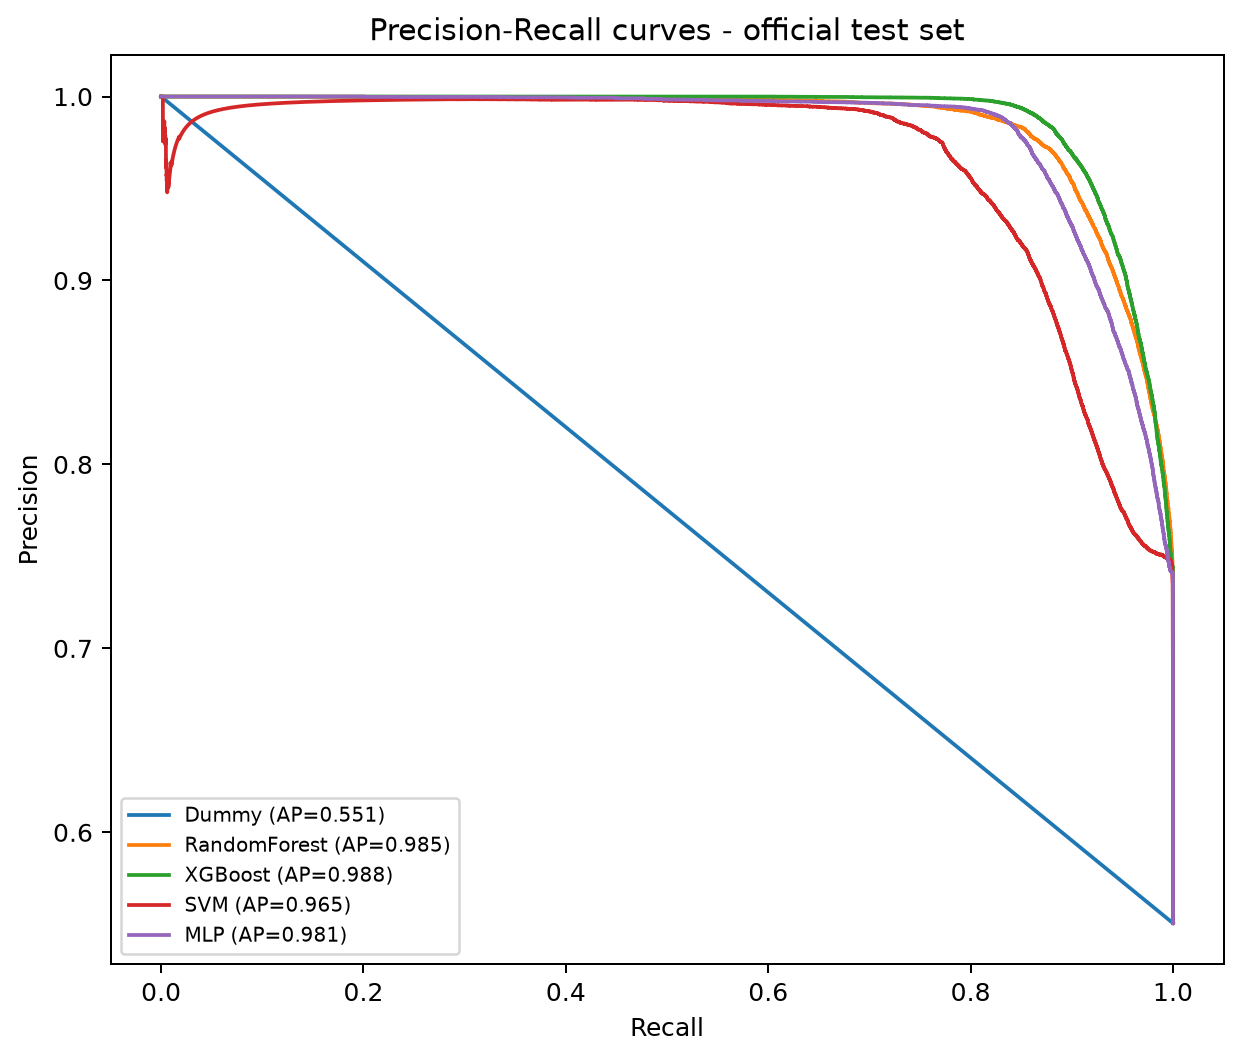
\includegraphics[width=0.48\textwidth]{figures/04_precision_recall_curves.png}
\caption{ROC curves and precision-recall curves on the official test set.}
\label{fig:rocpr}
\end{figure*}

Bootstrap resampling of fixed test predictions (1500 resamples per model) produced 95\% confidence intervals of F1 of $[0.8924, 0.8963]$ for XGBoost, $[0.8887, 0.8928]$ for Random Forest, and $[0.8873, 0.8914]$ for MLP. Official-test indices are resampled with replacement, and each metric is recomputed from the corresponding fixed model predictions, scores, and ground-truth labels; models are not retrained during this procedure. The independently estimated confidence intervals overlap marginally for XGBoost and Random Forest and do not overlap for XGBoost and MLP. Because these intervals were estimated independently and no paired bootstrap interval or paired hypothesis test of model differences was performed, they are interpreted descriptively rather than as evidence of statistically significant superiority. For the XGBoost demonstration model specifically, bootstrap intervals were also computed for ROC-AUC $[0.9831, 0.9843]$, PR-AUC $[0.9876, 0.9885]$, MCC $[0.7514, 0.7592]$, recall $[0.9823, 0.9847]$, and FPR $[0.2602, 0.2688]$, using 1500 valid bootstrap samples.

All four non-baseline models exhibit a false positive rate above one quarter of normal test traffic (26.5\%--40.0\%). Because recall for these models simultaneously exceeds 0.97, a high detection rate is being obtained at the cost of flagging a substantial share of normal connections; in an operational setting with far more normal than malicious traffic, this FPR could translate into a large volume of false alerts. A high ROC-AUC or PR-AUC therefore does not by itself indicate that a model's default operating point is suitable for deployment, and threshold selection against an operational false-alert budget would need to be studied separately from this benchmark comparison \cite{sommerpaxson2010closed}.

Comparing Table~\ref{tab:cv} with Table~\ref{tab:test} shows a consistent reduction in F1 from the descriptive training-set cross-validation to the official held-out partition (approximately 0.07--0.10 across all five models, including the Dummy baseline). The fact that this reduction also occurs for the label-blind Dummy baseline indicates that partition-level distribution and class-prevalence differences between the predefined UNSW-NB15 training and testing partitions contribute materially to the observed CV-to-test gap; this observation does not rule out additional model-specific overfitting in the trained classifiers. The predefined test set should therefore be treated as a substantially more challenging evaluation setting than the descriptive training-set CV suggests.

\subsection{Attack-wise Detection}
Table~\ref{tab:attackwise} and Fig.~\ref{fig:attackwise} show attack-wise detection counts and recall for the XGBoost demonstration model. The aggregate recall of 0.9835 masks a substantially lower recall for Fuzzers (0.8903, 665 missed of 6062), while Backdoor and Worms were fully detected in this run and Generic, Reconnaissance, and DoS all exceeded 0.998 recall. This heterogeneity confirms RQ2: aggregate binary metrics are insufficient to characterize model behavior across attack families, and the comparatively higher difficulty of Fuzzers is consistent with previously reported class overlap between Fuzzers and normal traffic in UNSW-NB15 \cite{zoghi2024overlap}.

\begin{table}[htbp]
\caption{XGBoost attack-wise binary detection recall}
\label{tab:attackwise}
\centering
\resizebox{\columnwidth}{!}{
\begin{tabular}{lrrrr}
\toprule
Attack family & n & Detected & Missed & Recall \\
\midrule
Fuzzers & 6062 & 5397 & 665 & 0.8903 \\
Analysis & 677 & 664 & 13 & 0.9808 \\
Shellcode & 378 & 375 & 3 & 0.9921 \\
Exploits & 11132 & 11074 & 58 & 0.9948 \\
DoS & 4089 & 4084 & 5 & 0.9988 \\
Reconnaissance & 3496 & 3494 & 2 & 0.9994 \\
Generic & 18871 & 18870 & 1 & 0.9999 \\
Backdoor & 583 & 583 & 0 & 1.0000 \\
Worms & 44 & 44 & 0 & 1.0000 \\
\bottomrule
\end{tabular}}
\end{table}

\begin{figure}[htbp]
\centerline{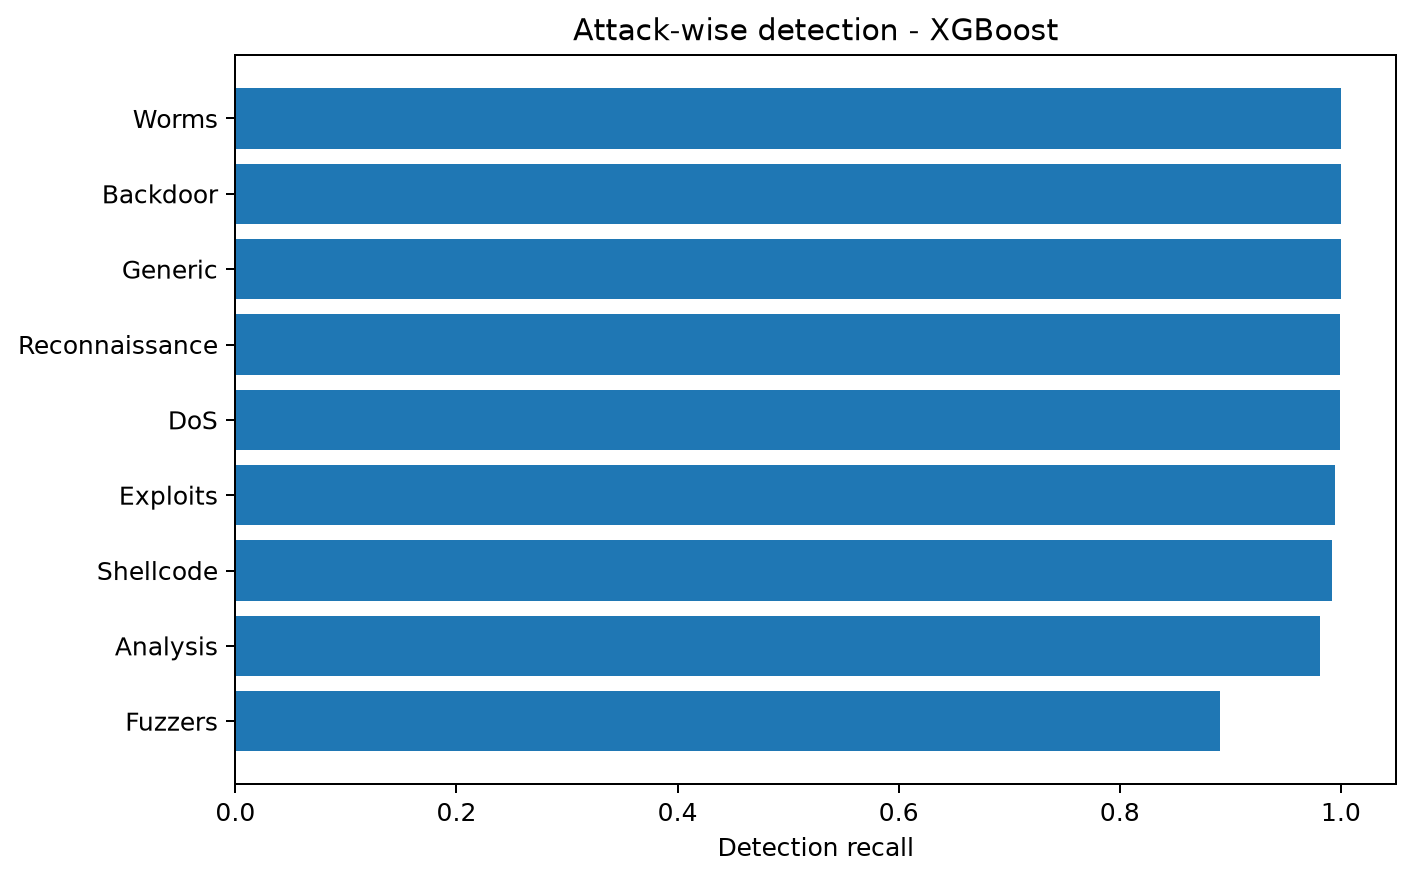
\includegraphics[width=\columnwidth]{figures/07_attackwise_recall.png}}
\caption{Attack-wise recall for the XGBoost demonstration model.}
\label{fig:attackwise}
\end{figure}

\subsection{Feature Importance}
Permutation importance for the XGBoost model was computed on 8000 deterministic official-test records (FULL profile) with 15 repeats and F1 scoring. Table~\ref{tab:importance} lists the ten highest-ranked features, and Fig.~\ref{fig:importance} shows the corresponding ranking. The strongest feature was \texttt{sttl} by a wide margin, followed by byte-count and packet-size features (\texttt{dbytes}, \texttt{dmean}, \texttt{sbytes}) and the connection-count feature \texttt{ct\_dst\_src\_ltm}. These results are diagnostic and model-specific; they should not be interpreted causally. XGBoost is retained as the model used for this analysis and for the Streamlit demonstrator because it obtained the numerically highest held-out F1 among non-baseline models in the FULL run, not because of an a priori preference.

\begin{table}[htbp]
\caption{Top permutation importances for XGBoost}
\label{tab:importance}
\centering
\resizebox{\columnwidth}{!}{
\begin{tabular}{lrr}
\toprule
Feature & Mean decrease & Std. \\
\midrule
\texttt{sttl} & 0.1055 & 0.0029 \\
\texttt{dbytes} & 0.0279 & 0.0012 \\
\texttt{dmean} & 0.0221 & 0.0009 \\
\texttt{sbytes} & 0.0221 & 0.0009 \\
\texttt{ct\_dst\_src\_ltm} & 0.0209 & 0.0015 \\
\texttt{smean} & 0.0173 & 0.0007 \\
\texttt{service} & 0.0145 & 0.0010 \\
\texttt{synack} & 0.0116 & 0.0007 \\
\texttt{ct\_dst\_sport\_ltm} & 0.0096 & 0.0012 \\
\texttt{ct\_dst\_ltm} & 0.0086 & 0.0008 \\
\bottomrule
\end{tabular}}
\end{table}

\begin{figure}[htbp]
\centerline{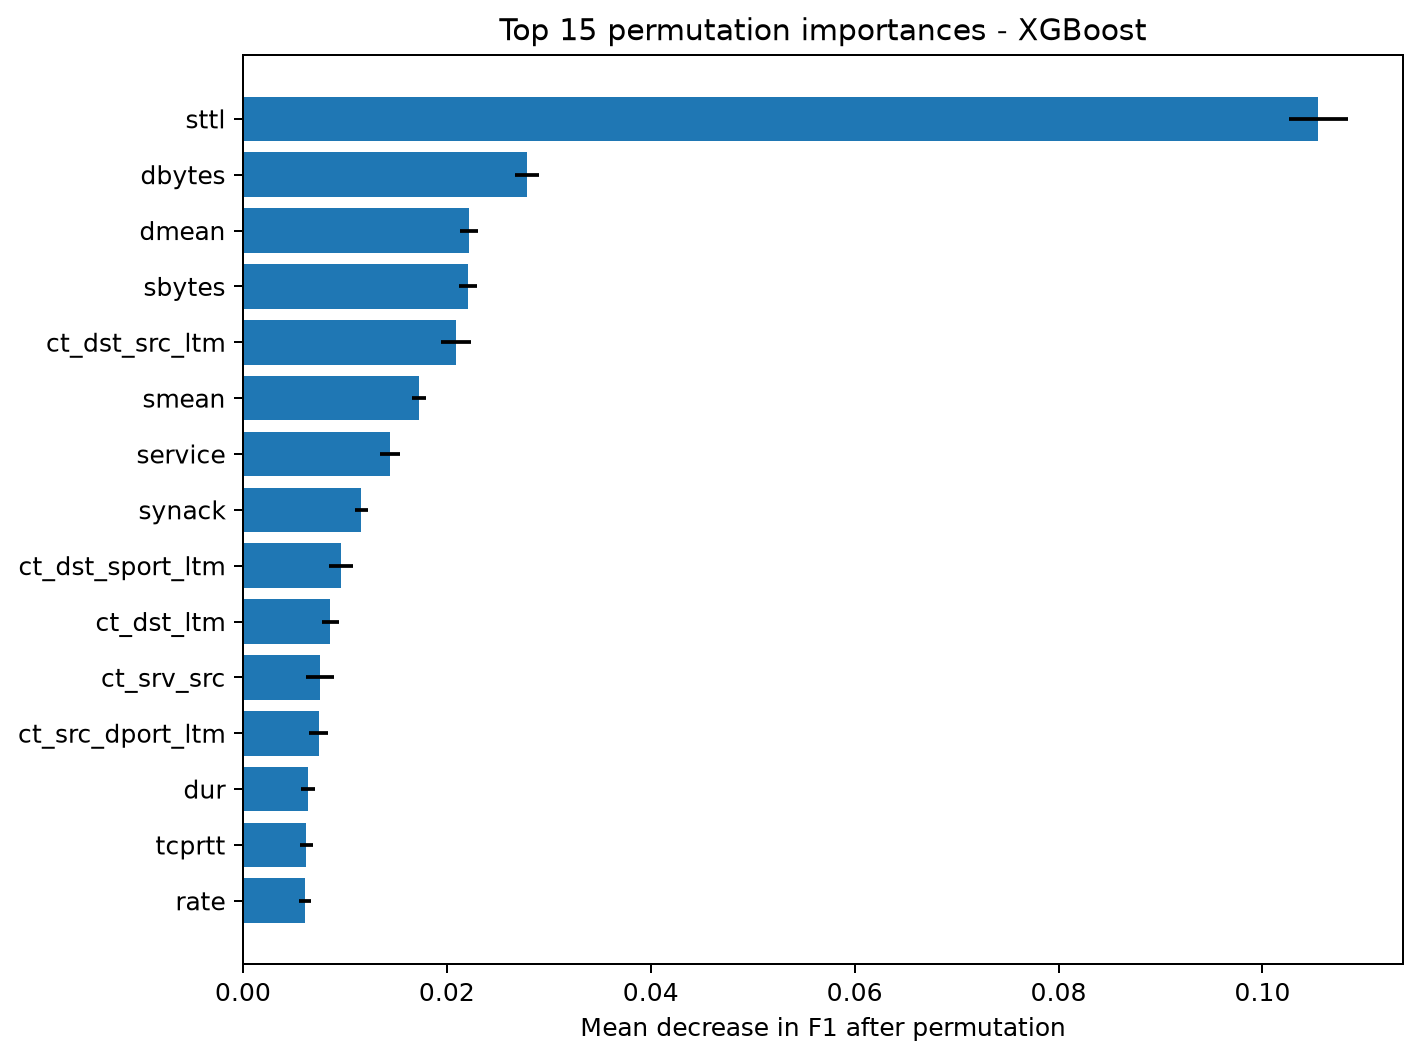
\includegraphics[width=\columnwidth]{figures/08_permutation_importance.png}}
\caption{Top permutation importances measured as mean decrease in F1.}
\label{fig:importance}
\end{figure}

\subsection{Unsupervised Analysis}
The clustering run sampled 15000 training records (FULL profile), encoded 189 dimensions, and retained 21 PCA components to preserve at least 95\% variance (95.00\% retained). Table~\ref{tab:clustering} summarizes the primary clustering outputs. k-Means with $k=2$ achieved silhouette 0.3335. The internally selected DBSCAN configuration used \texttt{eps=1.834593} and \texttt{min\_samples=10}, yielding 13 non-noise clusters, 3.18\% noise, and silhouette 0.2544; this silhouette is computed after excluding noise points, consistent with the internal, label-free selection procedure described in the Methodology. ARI and NMI remained low for both methods (at most 0.127), which is consistent with the exploratory rather than supervised nature of the clustering experiment: the recovered structure is not a close proxy for the binary attack label. Fig.~\ref{fig:clustering} visualizes the first two principal components together with the hidden binary labels, k-Means assignments, and DBSCAN assignments; labels are used only for this post-hoc visualization and never during fitting.

\begin{table}[htbp]
\caption{Consolidated clustering metrics}
\label{tab:clustering}
\centering
\resizebox{\columnwidth}{!}{
\begin{tabular}{lrrrrr}
\toprule
Algorithm & Clusters & Noise & Silhouette & ARI & NMI \\
\midrule
k-Means ($k=2$) & 2 & 0.0000 & 0.3335 & 0.1108 & 0.0816 \\
DBSCAN & 13 & 0.0318 & 0.2544 & 0.1274 & 0.1108 \\
\bottomrule
\end{tabular}}
\end{table}

\begin{figure*}[t]
\centering
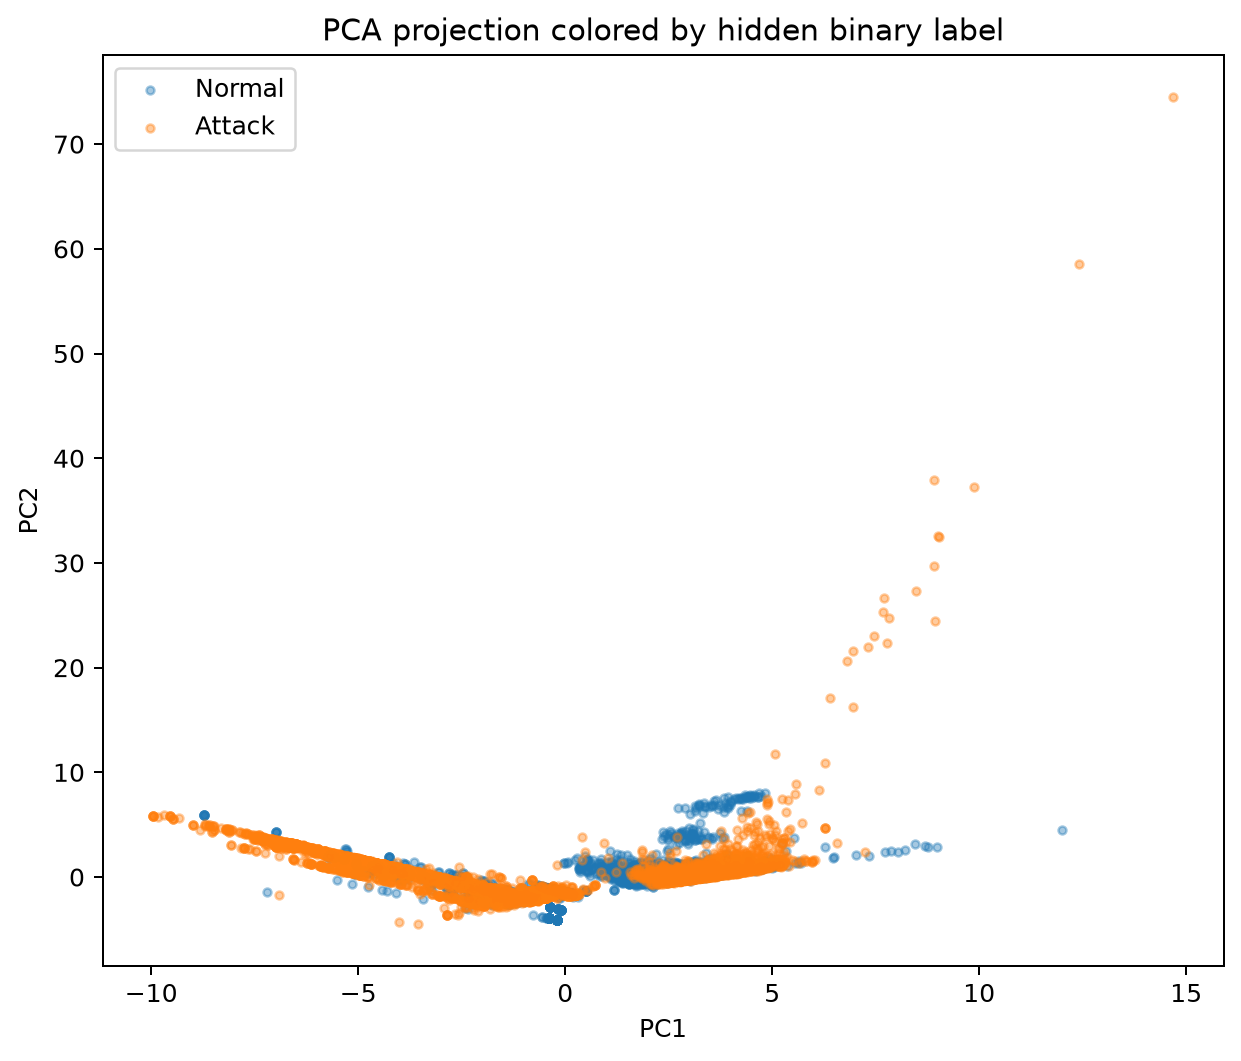
\includegraphics[width=0.32\textwidth]{figures/09_pca_true_labels.png}
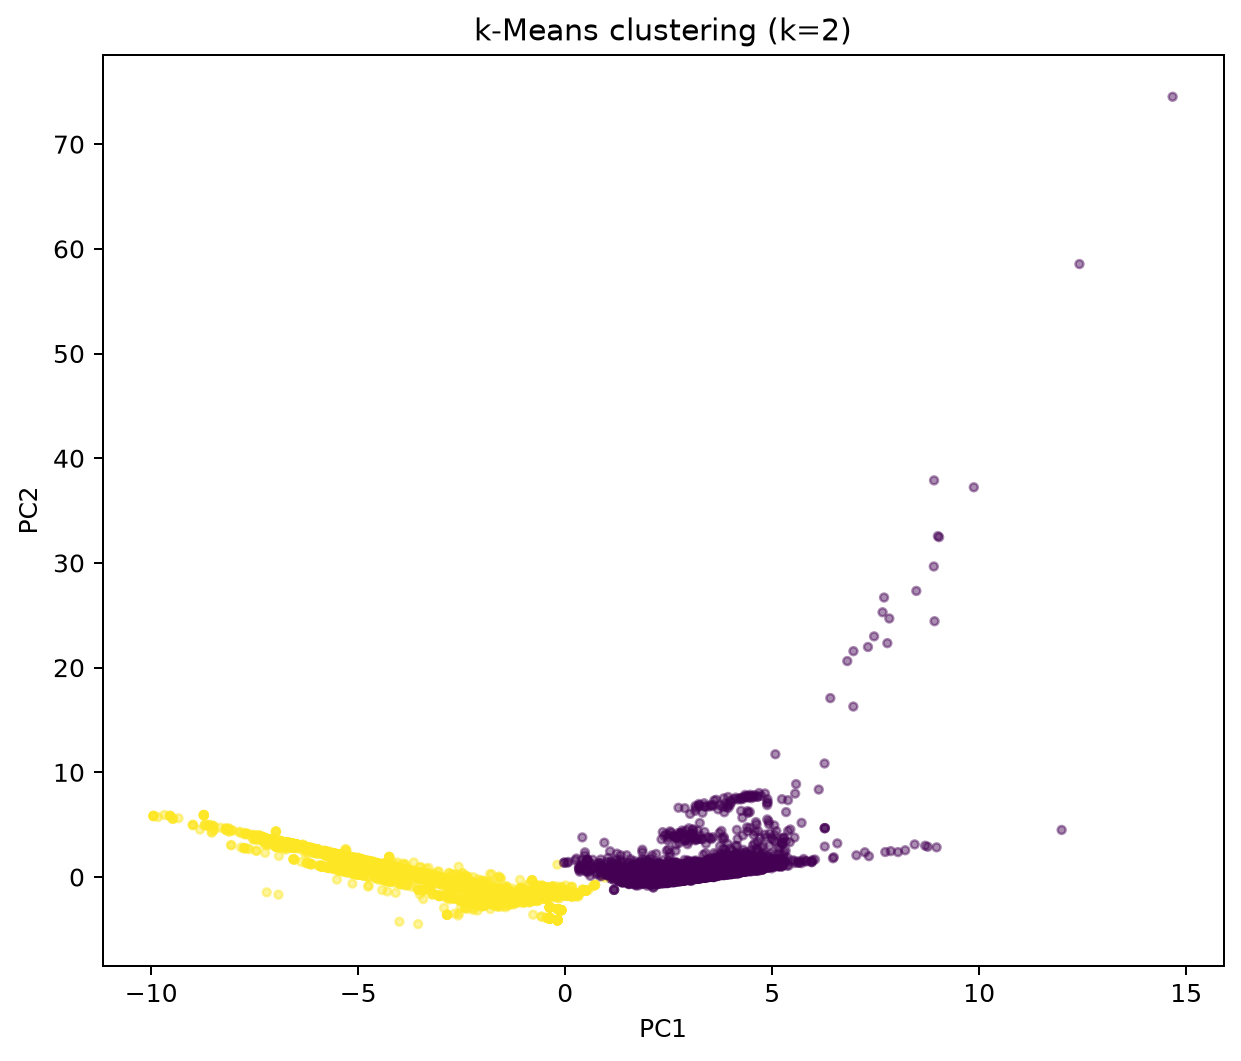
\includegraphics[width=0.32\textwidth]{figures/11_pca_kmeans.png}
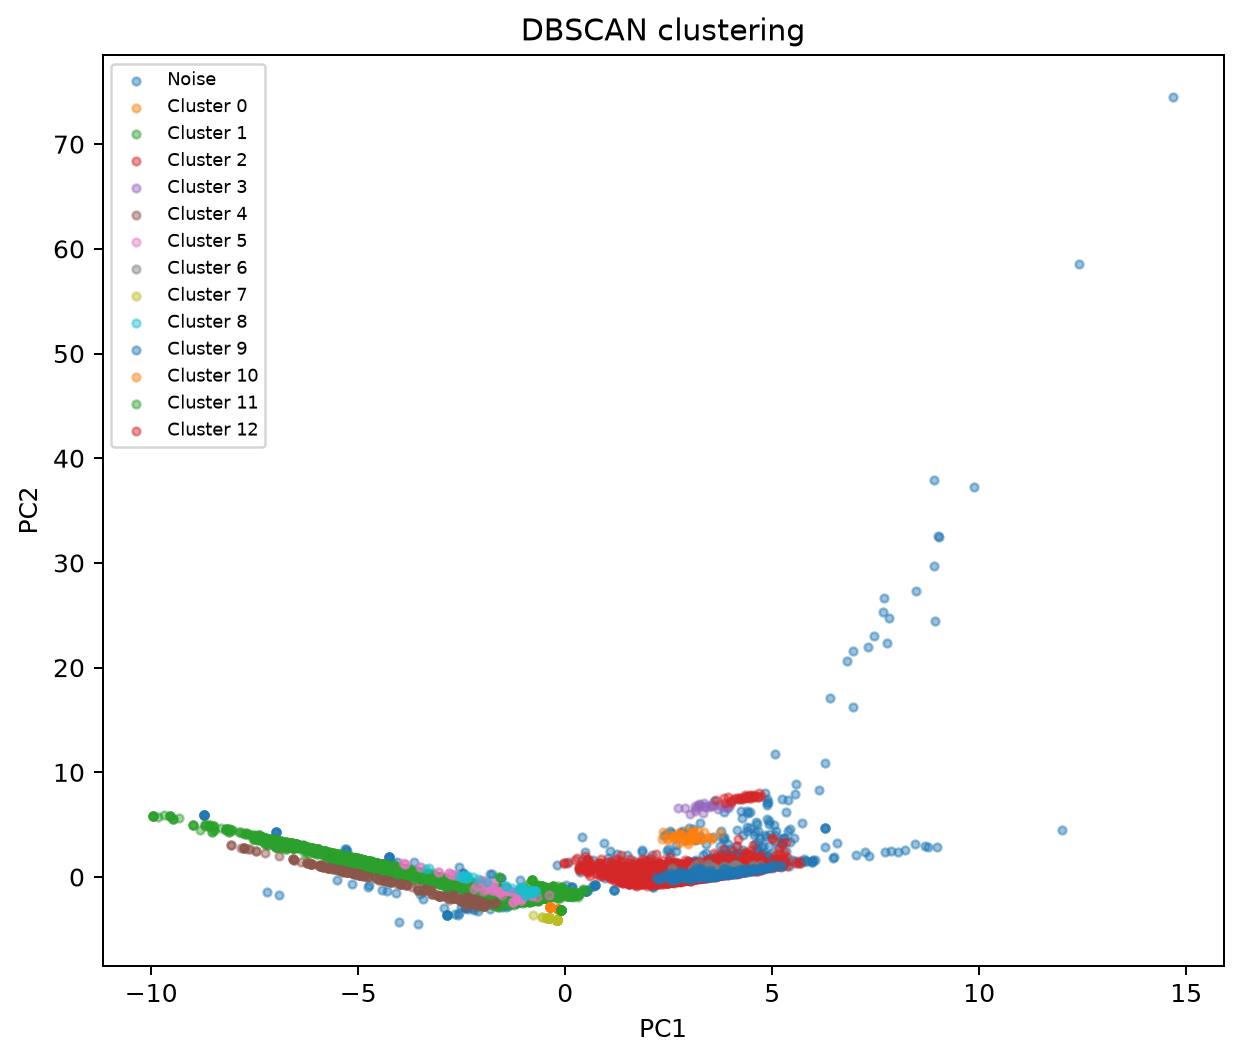
\includegraphics[width=0.32\textwidth]{figures/13_pca_dbscan.png}
\caption{Two-dimensional PCA visualization with hidden true labels, k-Means assignments, and DBSCAN assignments. Labels are used only for post-hoc visualization.}
\label{fig:clustering}
\end{figure*}

\subsection{Computational Efficiency}
Table~\ref{tab:efficiency} summarizes final fit time (a single fit on the complete training partition, separate from the hyperparameter-search procedure summarized in Table~\ref{tab:hyperparams}), median inference latency, and serialized artifact size for the FULL run. XGBoost gave the numerically highest test F1 with a final fit time of 4.10~s and a 2.24~MB serialized artifact -- markedly smaller than Random Forest's 35.87~MB, although larger than a more lightly tuned configuration would produce, because the FULL search selected 600 boosting rounds at depth 9. LinearSVC produced the smallest artifact overall (4.94~KB) and the fastest median per-record inference among non-baseline models (1.59~$\mu$s/record), but at a lower F1 and a higher FPR (39.95\%) than the tree-based and neural models. The Multilayer Perceptron had the longest final fit time (68.89~s), reflecting its larger selected hidden-layer configuration, yet produced a comparatively compact 0.71~MB artifact. These results illustrate RQ4's trade-off: no single model dominates simultaneously on predictive performance, artifact size, training cost, and inference cost.

\begin{table}[htbp]
\caption{Efficiency and artifact-size summary. Sizes are reported in MB unless noted otherwise.}
\label{tab:efficiency}
\centering
\resizebox{\columnwidth}{!}{
\begin{tabular}{lrrr}
\toprule
Model & Final fit time (s) & Inference ($\mu$s/record) & Size \\
\midrule
XGBoost & 4.10 & 2.49 & 2.24 MB \\
RandomForest & 14.83 & 3.09 & 35.87 MB \\
MLP & 68.89 & 4.41 & 0.71 MB \\
SVM & 7.33 & 1.59 & 4.94 KB \\
Dummy & 0.22 & 1.15 & 2.22 KB \\
\bottomrule
\end{tabular}}
\end{table}

\FloatBarrier

\section{Discussion}
The supervised results answer RQ1 by showing that XGBoost, Random Forest, and MLP are closely grouped on the official test set (F1 between 0.8893 and 0.8943), with bootstrap intervals that only marginally separate XGBoost from Random Forest and do not separate XGBoost from MLP by a wide margin either; LinearSVC trails clearly in both F1 and FPR. XGBoost is retained as the Streamlit demonstration model because it obtained the numerically highest held-out F1 among non-baseline models in the FULL run, not because the test set was used for hyperparameter tuning. Random Forest remains competitive, particularly in recall, but at a substantially larger serialized size (35.87~MB versus 2.24~MB).

RQ2 is supported by the attack-wise analysis. XGBoost appears strong in aggregate (recall 0.9835), yet Fuzzers recall (0.8903) is markedly lower than recall for Generic, Backdoor, Worms, DoS, and Reconnaissance, all of which exceed 0.998. This pattern is consistent with previously reported overlap between Fuzzers and normal-traffic feature distributions in UNSW-NB15 \cite{zoghi2024overlap}, and it reinforces that binary intrusion-detection studies should report at least post-hoc attack-family behavior when such metadata are available; otherwise, high global detection rates can obscure families that remain comparatively difficult.

RQ3 receives a cautious answer. k-Means and DBSCAN reveal some structure in the PCA representation -- DBSCAN's internally selected configuration recovered 13 non-noise clusters at a low 3.18\% noise fraction -- but post-hoc ARI and NMI remain low (at most 0.127) for both methods. This does not invalidate the clustering analysis; rather, it indicates that unsupervised structure in this representation is not a close substitute for the supervised binary label, and that clustering results should be read as exploratory evidence of traffic heterogeneity rather than as an alternative detector.

RQ4 shows a visible trade-off between predictive performance and efficiency. XGBoost gave the numerically strongest F1 with a moderate artifact size and fast inference; LinearSVC was the smallest and fastest model but the least accurate; MLP required the longest training time without a compensating accuracy advantage over XGBoost or Random Forest. None of the four non-baseline models achieves both the highest predictive performance and the smallest computational footprint simultaneously.

Two further observations qualify all of the above. First, F1 dropped by approximately 0.07--0.10 for every model, including the label-blind Dummy baseline, when moving from the descriptive training-set cross-validation to the official held-out test partition. Because this drop also occurs for the label-blind Dummy baseline, partition-level distribution and class-prevalence differences between the predefined UNSW-NB15 partitions contribute materially to the observed gap; this does not rule out additional model-specific overfitting in the trained classifiers. Second, every non-baseline model produced a false positive rate above one quarter of normal traffic. High ROC-AUC and recall in this benchmark should therefore not be read as evidence of operational readiness: prior work has shown that machine-learning intrusion detectors validated on closed, offline datasets do not necessarily generalize to live operational networks \cite{sommerpaxson2010closed}, and the false-alert volume implied by a 26--40\% FPR would need to be evaluated against a realistic normal-to-attack traffic ratio before any deployment claim could be supported.

\section{Limitations}
This study has several limitations. First, UNSW-NB15 was produced in a controlled cyber-range, so the results do not demonstrate performance in real operational networks. Second, the main task is binary attack detection; \texttt{attack\_cat} is metadata for post-hoc analysis and not a model input. Third, LinearSVC was chosen instead of a kernel SVM because of the size of the training set (approximately 175 thousand records), which would make kernel methods substantially more expensive. Fourth, hyperparameter search remains limited to 15 randomly sampled configurations per model over the search spaces in Table~\ref{tab:hyperparams}; a larger or exhaustive search could yield different selected configurations. Fifth, the unsupervised experiment is exploratory and is run on a bounded training-set sample (15000 records) rather than the full training partition. Sixth, PCA and clustering results are sensitive to representation choices, and DBSCAN is additionally sensitive to the \texttt{eps}/\texttt{min\_samples} parameterization and to sample size. Seventh, the bootstrap confidence intervals reported here compare models independently and do not constitute a formal paired statistical test of superiority. Finally, this project does not parse raw PCAP, ingest raw Syslog or NetFlow, monitor live traffic, or claim validation in SCADA, thermoelectric, or other Operational Technology environments.

\section{Conclusion}
This paper presented a reproducible classical-ML benchmark for UNSW-NB15, executed under the FULL experimental profile, that preserves the official train/test partition, avoids metadata leakage, and reports aggregate, attack-wise, and computational outcomes together. XGBoost obtained the numerically highest held-out F1 score (0.8943), with Random Forest and a Multilayer Perceptron close behind and LinearSVC trading lower predictive performance for the smallest artifact and fastest inference; bootstrap intervals indicate that the top three models are not separated by a wide margin. Attack-wise evaluation showed that Fuzzers remained comparatively more difficult to detect than other attack families despite strong aggregate performance, and every non-baseline model exhibited a false positive rate exceeding one quarter of normal traffic, underscoring that this benchmark characterizes controlled predictive behavior rather than operational deployment readiness. The unsupervised analysis identified exploratory structure -- most clearly an internally selected 13-cluster DBSCAN configuration with low noise -- that did not align strongly with hidden labels. Future work could evaluate these models on external or more recent intrusion-detection datasets, study performance under temporal or domain shift relative to the cyber-range conditions used here, extract features from operational traffic-capture pipelines rather than precomputed CSV records, calibrate decision thresholds against a realistic false-alert budget, and assess detection performance under more realistic deployment conditions.

\section{Data Availability}
The UNSW-NB15 dataset used in this study is publicly available from UNSW Sydney \cite{unswDatasetPage}. The experiments use the predefined \texttt{UNSW\_NB15\_training-set.csv} and \texttt{UNSW\_NB15\_testing-set.csv} partitions. Raw dataset files are not redistributed through the project repository because they are third-party data.

For reproducibility, the project repository provides the data acquisition and validation workflow together with \texttt{data/data\_manifest.json}, which records the SHA-256 hashes of the exact dataset files used in the reported experiments. The project repository is available at \url{https://github.com/PesquisaDoug/unsw-nb15-ml-benchmark}.

A preserved research release of the associated code, configuration, manifests, and paper artifacts is archived on Zenodo at \url{https://doi.org/<ZENODO_DOI>}.

\section{Code Availability}
The source code, experiment configurations, reproducibility manifests, generated tables and figures, and manuscript sources associated with this study are publicly available at \url{https://github.com/PesquisaDoug/unsw-nb15-ml-benchmark}.

The implementation is organized under \texttt{src/}, executable entry points under \texttt{scripts/}, experiment configuration under \texttt{configs/}, and manuscript resources under \texttt{paper/}. Both QUICK and FULL experimental profiles are supported; the results reported in this paper correspond to the FULL profile, reproducible through the documented entry points \texttt{scripts.run\_supervised}, \texttt{scripts.run\_clustering}, and \texttt{scripts.generate\_results}. Complete installation and reproduction instructions are provided in the repository README.

The version associated with this manuscript corresponds to Git revision \texttt{0c44383212677a3dfc4facb3a69a495bfce412f4}. A preserved archival snapshot of this release is available through Zenodo at \url{https://doi.org/<ZENODO_DOI>}.

\FloatBarrier

\bibliographystyle{IEEEtran}
\bibliography{references}

\end{document}
